\documentclass[../main.tex]{subfiles}
\begin{document}

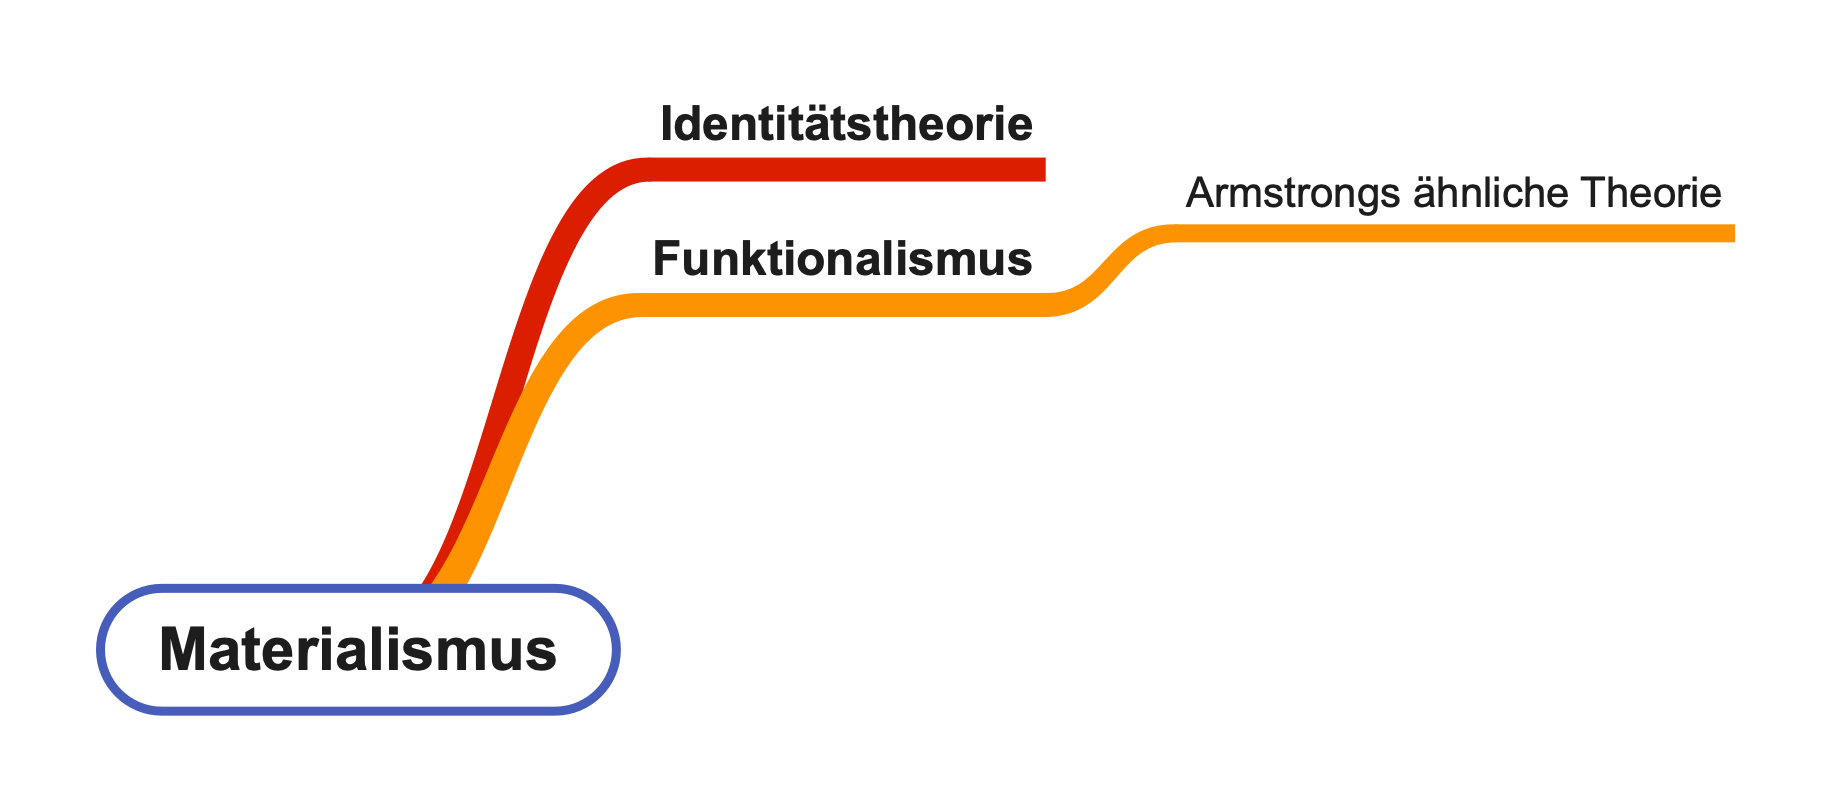
\includegraphics[width=\textwidth]{images/Materialismus_Uebersicht.png}

\section{Materialismus} 
\paragraph{These}
\begin{enumerate}
	\item Die Träger mentaler Eigenschaften sind physische Dinge (Körper, Gehirne)
	\item Mentale Eigenschaften/Zustände können auf physische Eigenschaften/Zustände zurückgeführt werden. 
\end{enumerate}

\section{Die (Geist-Gehirn-)Identitätstheorie}
Begründet und vertreten wurde die Theorie in den 1950er durch U. T. Place und J. J. C. Smart.
\paragraph{These} Jeder Empfindungszustand (in einigen Versionen jeder mentale Zustand) ist mit einem Gehirnzustand identisch. Entsprechende Identitätsaussagen sind \textit{synthetisch} und \textit{a posteriori}. 
\paragraph{Erklärung} 
\paragraph{Argumente}
\begin{enumerate}
	\item Smart: Es gibt keine überzeugende Argumente für den Dualismus
	\item Smart: Die Identiätstheorie kann die beobachteten Tatsachen ebensogut und konsistent erklären.
	\item Smart: Die methodologischen Prinzipien der Sparsamkeit und Einfachheit (Ockhams Razor) bevorzugen die Identitätstheorie (Smart: Der Dualismus hat viele irreduzible psychophysische Gesetze von seltsamer Art).
\end{enumerate}

\section{Der (analytische Realisierer-) Funktionalismus}  
Vertreten durch David Lewis (und auch J. J. C. Smart. und U. T. Place)
\paragraph{These} Jede Empfindung (d.h. jeder Typ von Empfindung) ist identisch mit einem physischen Zustand (d.h. mit einem physischen Zustandstyp).
\paragraph{Erklärung} Ganz grob gesagt besagt die Theorie, dass physischen Zustände durch ihre Funktion im Körper definiert sind. Wenn also die Empfindung von Schmerz zusammen mit dem Feuern der C-Fasern im Hirn, Geräuschen wie Stöhnen und dem Verziehen des Gesichtes einher gehen, so ist diese Schmerzempfindung gleich den beschrieben physischen Zuständen. 
\paragraph{Argumente}
\begin{enumerate}
	\item Lewis: Wenn (1) eine Empfindung eine bestimmte kausale Rolle spielt (analytisch) und gleichzeitig (2) ein physischer Zustand dieselbe kausale Rolle spielt, dann (3) ist der physische Zustand gleich der Empfindung.
		\begin{itemize}
			\item \textbf{kausale Rolle}: Beinhaltet die typischen Ursachen und Wirkungen für einen bestimmten Zustand. Dazu zählen alle peripheren Ereignisse wie Inputs (z.B. Reizung von Rezeptorzellen), Outputs (z.B. Bewegung) und der Einfluss von anderen Systemzuständen. Als Beispiel kann man Tanzen im Club nehmen nehmen; Inputs sind Musik und visuelle Eindrücke, Outputs sind die eigenen Bewegungen und Einflüsse sind positive Konotationen und Erfahrungen. All dies resultiert in einer Empfindung, die gleich dem physischen Zustand ist, in dem sich der Körper (und das Hirn) befindet.
			\item \textbf{analytische Natur der 1. Prämisse}: Lewis sagt, dass wir alltagssprachliche Platitüden über Empfindungszustände haben (z.B. <<Verletzung verursachen typischerweise Schmerzen>>). Aus diesen Platitüden lassen sich Definitionen von mentalen Ausdrücken ableiten (vereinfachte Definition von Schmerzzustand = derjenige, der (i) typischerweise von Verletzungen verursacht wird, (ii) typischerweise einher geht mit Schreien, Weinen und Gesichtsverzerrungen und (iii) typischerweise einen Zustand der Aufregung verursacht).
			\item \textbf{2. Prämisse}: Lewis rechtfertigt dies mit der kausalen Geschlossenheit der physischen Welt; da es sich bei der Ereignissen wie Schreien und Weinen um physische Phänomene handelt, muss es für sie eine physikalische Erklärung geben (eine, die ausschliesslich auf physische Ursachen verweist). Wir dürfen annehmen, dass es ein physischer Zustand ist, der die kausale Rolle spielt. 
		\end{itemize}
\end{enumerate}
\paragraph{Abgrenzung von Identitätstheorie} Als Begründung benutzt Lewis keine (schwache) Sparsamkeitsbegründung. 
\paragraph{Abgrenzung und Namensgebung} erfolgt anhand folgender Erklärungen: 
\begin{itemize}
	\item Weil Lewis' kausale Rollen auch als funktionale Rollen bezeichnet werden, hat sich der Name <<Funktionalismus>> gebildet
	\item Weil (1. Prämisse) Lewis Empfindungen mittels funktionaler Rollen definiert und somit eine funktionale Analyse von Empfindungen möglich wird, hat sich der Namenszusatz <<analytischer Funktionalismus>> gebildet.
	\item Weil die kausale Rolle etwas realisiert, wird der Anhang <<Realisierer>> angeführt. 
\end{itemize}


\subsection{Armstrong's ähnliche Theorie}
Gleichzeitig mit Lewis hat D. M. Armstrong eine ähnliche Position entwickelt. Diese unterscheidet sich jedoch darin, dass die Theorie von Empfindungen auf alle mentalen Zustände ausgeweitet sind (Lewis schliesst sich dem später an). Des weiteren äussert Armstrong irgendwann Zweifel an der Analytizität der funktionalen Charakterisierung, die Lewis nicht teilt. 

\subsection{Andere Varianten}
Es gibt den Psychofunktionalismus/Synthetischer Funktionalismus (im Gegensatz zum Analytischen Funktionalismus), den Rollen-Funktionalismus (im Gegensatz Realisier-Funktionalismus von Lewis) und Weiterentwicklungen des Funktionalismus wie Teleofunktionalismus oder der computationale Funktionalismus. 


\end{document}